\begin{frame}{Introduction}

	\begin{minipage}[c][.23\textheight]{.8\textwidth}
		\begin{itemize}
			\itemfill
			\item in early 90s all SM particles except H and t-quark discovered
			\item beauty discovery \ra weak isospin partner was undoubted
			\item quark masses are fundamental parameters in the SM
		\end{itemize}
	\end{minipage}
	\begin{minipage}{.18\textwidth}
		\fig{B1}{.2}
	\end{minipage}
	
	\begin{itemize}\itemfill
		\item early estimates: $\z{m}_{\z{t}} \approx 3 \z{m}_{\z{b}} \approx \SI{15}{\giga\electronvolt}$
		\item many new accelerator could only push limits higher:
		\item TRISTAN ($e^+e^-$) at KEK (Tsukuba, Japan) with $\sqrt{s} = \SI{61.4}{\giga\electronvolt}$ \ra \SI{30.2}{\giga\electronvolt}
		\item Sp$\overline{\z{p}}$S at CERN with $\sqrt{s} = \SI{630}{\giga\electronvolt}$ \ra \SI{69}{\giga\electronvolt}
		\item SLC ($e^+e^-$) at Stanford and LEP ($e^+e^-$) at CERN \ra $\sfrac{1}{2} \z{m}_{\z{t}}$
		\item hadron collider needed (\ra Tevatron)
	\end{itemize}
	
\end{frame}
%%%%%%%%%%%%%%%%%%%%%%%% FRAME 1 %%%%%%%%%%%%%%%%%%%%%%%%%%%%%%%
\begin{frame}{Decay Channels (1)}

	\begin{itemize}\itemfill
		\item estimate on $\z{m}_{\z{t}}$ in 1994: \SI{\sim180}{\giga\electronvolt}
		\item prior to discovery: behaviour completely predicted by SM
		\item $\z{m}_{\z{t}} > \z{m}_{\z{W}}$ \ra main decay channel (\SI{\sim96}{\%}):\ka{\usebeamercolor[fg]{title}\textbf{t\ch{->}$\z{W}^+\z{b}$}}
		\begin{equation*} \Upgamma_{\z{t}} = \frac{\z{G}_{\z{F}}\z{m}_{\z{t}}^{3}}{8\uppi\sqrt{2}}\left(1 - \frac{\z{m}_{\z{W}}^{2}}{\z{m}_{\z{t}}^{2}}\right)^{2}\left(1 + 2\frac{\z{m}_{\z{W}}^{2}}{\z{m}_{\z{t}}^{2}}\right)\end{equation*}
		\item width for the expected mass: \SI{\sim1}{\giga\electronvolt} \ra decay before hadronisation
	\end{itemize}
	
	\begin{figure}\vspace*{-10pt}
		\centering
		\subfig[.3]{tWbq}{.25}{\SI{\sim67}{\%}}
		\subfig[.3]{tWbl}{.25}{\SI{\sim33}{\%}}
	\end{figure}\vspace*{-10pt}
	
	\begin{itemize}\itemfill
		\item leptonic decay equally splits up into $e$, $\upmu$ and $\uptau$
	\end{itemize}

\end{frame}
%%%%%%%%%%%%%%%%%%%%%%%% FRAME 2 %%%%%%%%%%%%%%%%%%%%%%%%%%%%%%%
\begin{frame}{Decay Channels (2)}

	\begin{itemize}\itemfill
		\item top mostly pair produced via $\z{q}\overline{\z{q}}$\ch{->}$\z{t}\overline{\z{t}}$ or gluon fusion: $\z{g}\z{g}$\ch{->}$\z{t}\overline{\z{t}}$  
		\item main decay of the top pair: $\z{t}\overline{\z{t}}$\ch{->}$\z{W}^+\z{b}\z{W}^-\overline{\z{b}}$
		\item b decay:
	\end{itemize}
	
	\begin{figure}\vspace*{-10pt}
		\centering
		\subfiga[.3]{BDec2}{.25}\hspace*{10pt}
		\subfiga[.4]{BDec1}{.25}
	\end{figure}
	
	\begin{itemize}\itemfill
		\item typical signals:
		\begin{itemize}
			\item 2 b-jets + dilepton ($e^+e^-$, $\upmu^+\upmu^-$, $e^+\upmu^-$, $\upmu^+e^-$)
			\item 2 b-jets + single lepton + two jets
			\item 2 b-jets + 4 jets
		\end{itemize}
		\item huge background on pure QCD process due to other more common QCD processes
		\item how to discriminate b-jets from other jets?
	\end{itemize}

\end{frame}
%%%%%%%%%%%%%%%%%%%%%%%% FRAME 3 %%%%%%%%%%%%%%%%%%%%%%%%%%%%%%%
\begin{frame}{B-Tagging}

	\begin{itemize}\itemfill
		\item most jets from light partons (u,d,s) or gluons
		\item lower rates from c, and b quarks
		\item interesting physics from b \ra top, higgs, supersymmetry or new phenomena
		\item b longer lifetime than other partons
		\item look for secondary vertices (away from primary vertex \ra interaction point)
		\item first reconstruct primary vertex:
		\begin{itemize}
			\item cluster all tracks together and determine likelihood they origin from common vertex
			\item vertex with highest p$_{\z{T}}$ = primary vertex
		\end{itemize}
		
	\end{itemize}
	\begin{minipage}[c][.22\textheight]{.5\textwidth}
		\begin{itemize}
			\item background for secondary vertices (mostly from light flavoured jets)
			\begin{itemize}
				\item K-short Meson
				\item lambda Baryon 
				\item photon conversion 
			\end{itemize}
		\end{itemize}
	\end{minipage}
	\begin{minipage}{.45\textwidth}
		\fig{BTag}{.4}
	\end{minipage}



\end{frame}
%%%%%%%%%%%%%%%%%%%%%%%% FRAME 4 %%%%%%%%%%%%%%%%%%%%%%%%%%%%%%%
\begin{frame}{$\z{t}\overline{\z{t}}$ Cross Section}

	\vspace*{-10pt}\fig{ttcs}{.65}\vspace*{-10pt}
	
	\begin{itemize}\itemfill
		\item cross section extracted from SM
		\item Tevatron Lumi in 1995: \SI{10e30}{\per\centi\meter\squared\per\second}
		\begin{equation*} \z{R}_{\z{t}\overline{\z{t}}} = \upsigma_{\z{t}\overline{\z{t}}}\mathscr{L} = \SI{.1}{\hertz}\end{equation*}

	\end{itemize}

\end{frame}
\subsection{Discovery at CDF}
%%%%%%%%%%%%%%%%%%%%%%%% FRAME 5 %%%%%%%%%%%%%%%%%%%%%%%%%%%%%%%
\begin{frame}{Discovery Paper (1)}
	\fig{TDis1}{.84}
\end{frame}
%%%%%%%%%%%%%%%%%%%%%%%% FRAME 6 %%%%%%%%%%%%%%%%%%%%%%%%%%%%%%%
\begin{frame}{Discovery Paper (2)}
	\fig{TDis2}{.84}
\end{frame}
%%%%%%%%%%%%%%%%%%%%%%%% FRAME 7 %%%%%%%%%%%%%%%%%%%%%%%%%%%%%%%
\begin{frame}{CDF Detector (1)}[plain]
	\begin{tikzpicture}[remember picture,overlay]
		\node[at=(current page.center)] {
			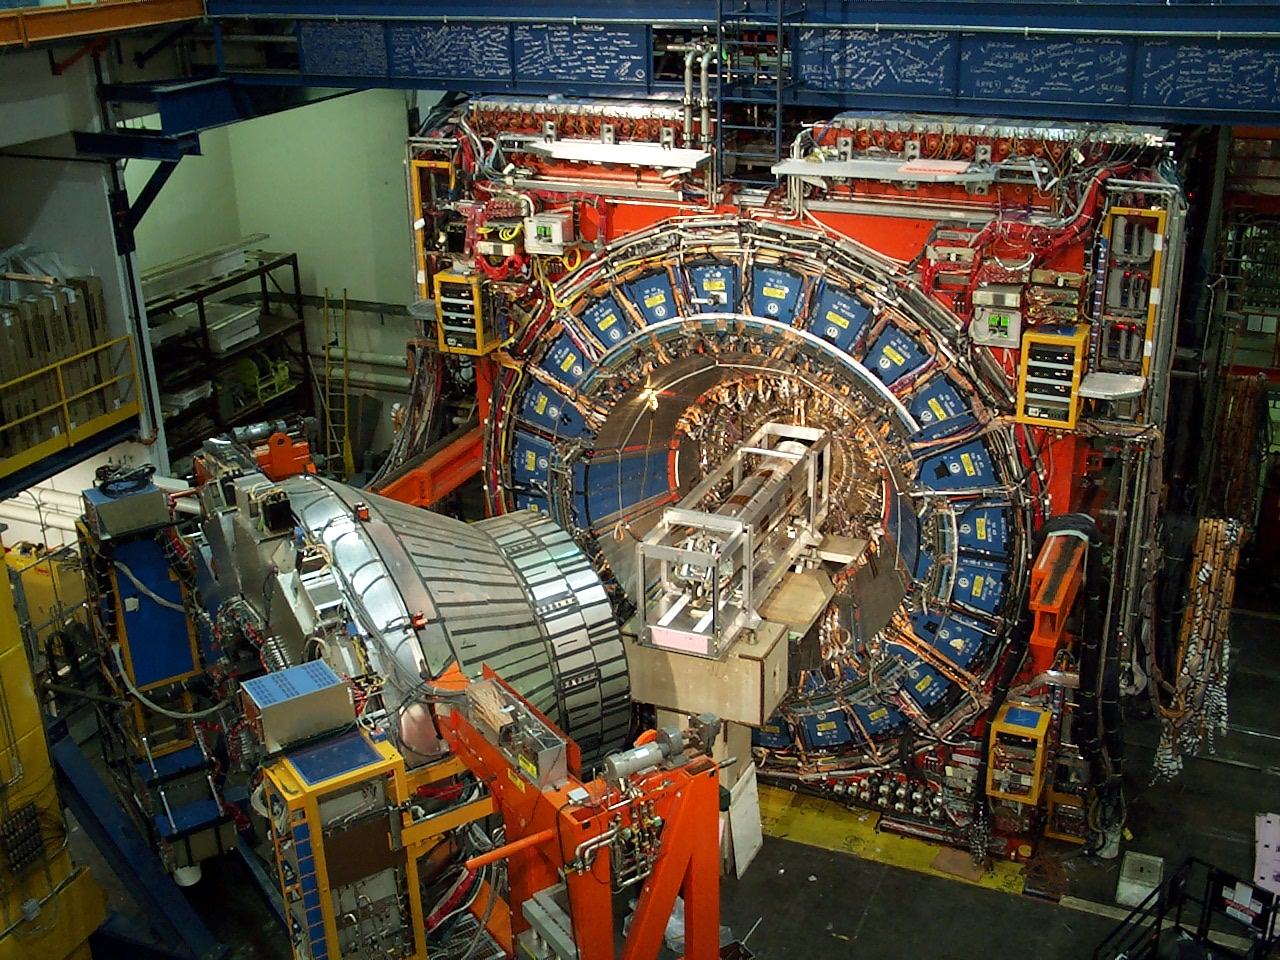
\includegraphics[width=\paperwidth]{cdfdet}
		};
	\end{tikzpicture}
\end{frame}
%%%%%%%%%%%%%%%%%%%%%%%% FRAME 8 %%%%%%%%%%%%%%%%%%%%%%%%%%%%%%%
\begin{frame}{CDF Detector}
	\fig{CDFDet1}{.84}
\end{frame}
%%%%%%%%%%%%%%%%%%%%%%%% FRAME 9 %%%%%%%%%%%%%%%%%%%%%%%%%%%%%%%
\begin{frame}{Introduction}
	
	\begin{itemize}\itemfill
		\item paper from 1994 with estimate on mass and cross section
		\item using dataset of \SI{19}{\per\pico\barn} + \SI{47}{\per\pico\barn} (\ra $\sim$ 400 events)
		\item looking at two decay channels
		\begin{itemize}
			\item dilepton
			\item lepton + jets
		\end{itemize}
		\item both data samples subsets of events with isolated leptons with high $P_{T}>\SI{20}{\giga\electronvolt}$
		\item cut on invariant mass of dilepton $\SI{75}{\giga\electronvolt}<\z{m}_{\z{I}}<\SI{105}{\giga\electronvolt}$ \ra exclude Z events
		\item main background reduction by b-tagging
		\begin{itemize}
			\item reconstruction of secondary vertices from b decay in SVX \ra SVX tag 
			\item finding additional leptons from b decay in ECAL \ra SLT tag 
		\end{itemize}
	\end{itemize}

\end{frame}
%%%%%%%%%%%%%%%%%%%%%%%% FRAME 10 %%%%%%%%%%%%%%%%%%%%%%%%%%%%%%%
\begin{frame}{Lepton + Jets Channel}
	
	\underline{\textbf{SVX tagging:}}\vspace*{5pt}
	\begin{itemize}\itemfill 
		\item search for secondary vertices with three ore more tracks
		\item then search for two ore more tracks with more stringed track and vertex quality
		\item efficiency estimated by $e$, $\upmu$ samples with enriched b decays (\SI{96}{\%} agreement to MC)
		\item tagging efficiency: \SI{42\pm5}{\%}
	\end{itemize}
	
	\begin{minipage}[c][.35\textheight]{.64\textwidth}
	 	\begin{itemize}\itemfill
			\item backgrounds:
			\begin{itemize}
				\item recoil of heavy quark pairs against W 
				\item mistags
			\end{itemize}
	 	 	\item for $\z{W}+\ge3$ jets: observation of \SI{27}{tags} with bg of \SI{6.7\pm2.1}{tags}
	 	 	\item decay lifetime of SVX tags agrees well with MC
	 	\end{itemize}
	\end{minipage}
	\begin{minipage}{.33\textwidth}
		\fig{CDFRes1}{.45}
	\end{minipage}

\end{frame}
%%%%%%%%%%%%%%%%%%%%%%%% FRAME 11 %%%%%%%%%%%%%%%%%%%%%%%%%%%%%%%
\begin{frame}{Dilepton Channel}
	
	\begin{minipage}[c][.35\textheight]{.64\textwidth}
		\begin{itemize}\itemfill 
			\item major backgrounds:
			\begin{itemize}
				\item Drall-Yan process
				\item Z\ch{->}$\uptau\uptau$
				\item misidentified hadrons
				\item WW, b$\overline{\z{b}}$
			\end{itemize}
			\item first three bg calculated by data and last two by MC
		\end{itemize}
	\end{minipage}
	\begin{minipage}{.33\textwidth}
		\fig{DrellYan}{.3}
	\end{minipage}
	
	\begin{itemize}\itemfill
		\item cuts:
		\begin{itemize}
			\item $\cancel{\z{E}}_{\z{T}}\ge\SI{10}{\giga\electronvolt}$
			\item number of jets $\ge2$
		\end{itemize}
		\item reduces Drell-Yan bg (very little $\cancel{\z{E}}_{\z{T}}$)
		\item correct for jet energy mismeasurement
	\end{itemize}

\end{frame}
%%%%%%%%%%%%%%%%%%%%%%%% FRAME 12 %%%%%%%%%%%%%%%%%%%%%%%%%%%%%%%
\begin{frame}{Results}

	\begin{table}
		\centering
		\begin{tabular}{lccc}
			\hline\hline
			\textbf{Channel}		&	\textbf{SVX}	& \textbf{SLT}		& \textbf{Dilepton}	\\\hline
			Observed				&	\SI{27}{tags}	& \SI{23}{tags}		& \SI{6}{events}	\\\hline
			Expected background		&	\SI{6.7\pm2.1}{}& \SI{15.4\pm2.0}{}	& \SI{1.3\pm0.3}{}	\\\hline\\[-10pt]
			Background probability	&	\SI{2e-5}{}		& \SI{6e-2}{}		& \SI{3e-3}{}		\\\hline\hline
		\end{tabular}
	\end{table}

	\begin{itemize}\itemfill
		\item combined likelihood of the background fluctuating up: \SI{1e-6}{} (\SI{4.8}{\upsigma})
	\end{itemize}

\end{frame}
%%%%%%%%%%%%%%%%%%%%%%%% FRAME 13 %%%%%%%%%%%%%%%%%%%%%%%%%%%%%%%
\begin{frame}{Mass Reconstruction}
	
	\begin{itemize}\itemfill
		\item kinematically mass reconstruction by use of single lepton + 4 jet events
		\item \ttb\ch{->}WbW$\overline{\z{b}}$\ch{->}$\z{q}\overline{\z{q}}$b$\ell\upnu\overline{\z{b}}$
		\item predicted mix of \SI{30}{\%} \ttb\ and \SI{70}{\%} W + jets bg (yellow)
		\item reducing bg by applying SVX and SLT tags
		\item get best top mass by using MC with W + jets bg and varying the top mass
	\end{itemize}
	
	\begin{figure}\vspace*{-5pt}
		\centering
		\subfig{CDFRes2}{.4}{before b-tagging}
		\subfig{CDFRes3}{.4}{after b-tagging}
	\end{figure}\vspace*{-20pt}
	
\end{frame}
%%%%%%%%%%%%%%%%%%%%%%%% FRAME 13 %%%%%%%%%%%%%%%%%%%%%%%%%%%%%%%
\begin{frame}{Combined Results}
	
	\begin{itemize}\itemfill
		\item combined signal size and mass distribution
		\item probability for and upward fluctuation of the bg: 
		{\usebeamercolor[fg]{title}\begin{equation*} \z{\textbf{P}}_{\z{\textbf{c}}} = \textbf{\SI{3.7e-7}{} (\SI{5.0}{\upsigma})} \end{equation*}}
		\item reconstructed mass:
		{\usebeamercolor[fg]{title}\begin{equation*} \z{\textbf{m}}_{\z{\textbf{top}}} = \textbf{\SI[parse-numbers=false]{176\pm8\pm10}{\giga\electronvolt\per c^2}} \end{equation*}}
		\item cross section:
		{\usebeamercolor[fg]{title}\begin{equation*} \mathbf{\upsigma}_{\z{\textbf{t}}\overline{\z{\textbf{t}}}} = \textbf{6.8}^{\textbf{+3.6}}_{\textbf{-2.4}}\, \z{\textbf{pb}} \end{equation*}}
	\end{itemize}
	
\end{frame}
